%------------------------------------------------------------------------------
% Template file for the submission of papers to IUCr journals in LaTeX2e
% using the iucr document class
% Copyright 1999-2013 International Union of Crystallography
% Version 1.6 (28 March 2013)
%------------------------------------------------------------------------------

\documentclass[pdf]{iucr}              % DO NOT DELETE THIS LINE
%\documentclass[preprint]{iucr} 
\usepackage{graphicx}
\usepackage{color}
\usepackage{ulem}
\usepackage{multicol}
%\usepackage{hyperref}


     %-------------------------------------------------------------------------
     % Information about journal to which submitted
     %-------------------------------------------------------------------------
     \journalcode{S}              % Indicate the journal to which submitted
                                  %   A - Acta Crystallographica Section A
                                  %   B - Acta Crystallographica Section B
                                  %   C - Acta Crystallographica Section C
                                  %   D - Acta Crystallographica Section D
                                  %   E - Acta Crystallographica Section E
                                  %   F - Acta Crystallographica Section F
                                  %   J - Journal of Applied Crystallography
                                  %   M - IUCrJ
                                  %   S - Journal of Synchrotron Radiation

\begin{document}                  % DO NOT DELETE THIS LINE

     %-------------------------------------------------------------------------
     % The introductory (header) part of the paper
     %-------------------------------------------------------------------------

     % The title of the paper. Use \shorttitle to indicate an abbreviated title
     % for use in running heads (you will need to uncomment it).

\title{TomoPy: A framework for the analysis of synchrotron tomographic data}
%\shorttitle{Short Title}

     % Authors' names and addresses. Use \cauthor for the main (contact) author.
     % Use \author for all other authors. Use \aff for authors' affiliations.
     % Use lower-case letters in square brackets to link authors to their
     % affiliations; if there is only one affiliation address, remove the [a].

\cauthor{Do\v{g}a}{G\"{u}rsoy}{dgursoy@aps.anl.gov}{} 
\author{Francesco}{De Carlo}
\author{Xianghui}{Xiao}
\author{Chris}{Jacobsen}


\aff{Advanced Photon Source, Argonne National Laboratory, 9700 S.~Cass Ave., Argonne IL 60439-4837 \country{USA}}


     % Keywords (required for Journal of Synchrotron Radiation only)
     % Use the \keyword macro for each word or phrase, e.g. 
     % \keyword{X-ray diffraction}\keyword{muscle}

\keyword{tomopgraphy}
\keyword{x-ray imaging}
\keyword{phase retrieval}

\hyphenpenalty=10000

\maketitle                        % DO NOT DELETE THIS LINE

\begin{synopsis}
Supply a synopsis of the paper for inclusion in the Table of Contents.
\end{synopsis}

\begin{abstract}
Analysis of large tomographic datasets at synchrotron light sources including X-ray transmission tomography, X-ray fluorescence microscopy and X-ray diffraction tomography is becoming progressively more challenging due to the increasing data acquisition rates that new technologies in X-ray sources and detectors enable. The next generation of synchrotron facilities that are currently under design or construction throughout the world will provide diffraction limited X-ray sources and is expected to boost the current data rates by several orders of magnitude and stressing the need for the development and integration of efficient analysis tools more than ever. Here we describe in detail an attempt to provide such a collaborative framework for the analysis of synchrotron tomographic data that has the potential to unify the effort of different facilities and beamlines performing similar tasks. The proposed Python/C++ based framework is open-source, platform and data format independent,  having multiprocessing capability and supports functional programming that many researchers prefer. This collaborative platform could affect all major synchrotron facilities where new effort is now dedicated into developing new tools that can be deployed at the facility for real time processing, as well as distributed to users for off site data processing.
\end{abstract}


\section{Introduction}

Analysis of large tomographic datasets at synchrotron light sources including X-ray transmission tomography (XCT), X-ray fluorescence microscopy (XFM) and X-ray diffraction tomography (XDT) is becoming progressively more challenging  due to the increasing data acquisition rates that new technologies in X-ray sources and detectors enable. The next generation of synchrotron facilities that are currently under design or construction throughout the world will provide diffraction limited X-ray sources and are expected to boost the current data rates by several orders of magnitude, thereby stressing the need for the development and integration of automated and efficient analysis tools more than ever. 

It is often the case that some users collect data at different facilities to take advantage of specific instrument characteristics and specifications, but they are left alone integrating this data with the available or home-grown software tools. However, there are strong similarities within the same class of instruments that are not systematically utilized to build a coordinated software development platform or framework where each facility and user group can take advantage from or contribute in, ultimately saving on-site resources by sharing the computing tasks with the user community. 

Here we describe in detail an attempt to provide such a collaborative framework for the analysis of synchrotron tomographic data that has the potential to serve the needs of different facilities and beamlines performing similar tasks. The basic principles of this Python-based open-source framework, called TomoPy (\texttt{http://www.aps.anl.gov/tomopy/}), include ease of collaborative development of scripts, platform and data format independence, modularity,  and support for a functional programming style that many researchers prefer. In the following sections, we will provide a brief background on the analysis of tomographic data at synchrotrons, and then shortly introduce the framework by describing the model structure together with the currently available methods. 


\section{Background}

When it comes to the digital storage of tomographic experimental data and the development of analysis tools at synchrotron light sources around the world, the situation is very heterogeneous. As different research teams and instruments have grown at various facilities, they have often developed local data and analysis models based on the instrument hardware specificity and often drawing upon the particular preferences of a scientist writing software. 

Many tomographic analysis tools utilize licensed (and often expensive) software packages like Matlab (The MathWorks, Inc.) and IDL (Exelis VIS), while others rely on specific (and often complex to maintain) computing infrastructure like MPI-based CPU or GPU clusters. This diversity and specialization hampers widespread delivery of an integrated development environment and limits its long term use. On the other hand, modern chip design shows a clear trend toward integration of multiple processor cores, thus permitting concurrency without a need for a dedicated cluster. The availability of inexpensive multi-core CPU workstations and the reduced cost of computer memory allow to considerably simplify the computing infrastructure required to process tomographic data \cite{rivers_spie_2012}, and make the development of single workstation tools able to perform most computing tasks at reasonable times. Besides, it allows the analysis to be performed on an off-site location, freeing on-site computational resources for other tasks. 

This transition is affecting all major synchrotron facilities where new effort is now dedicated into developing tools that can be deployed at the facility for real time processing as well as distributed to users for off-site data processing. We believe this will pave the way for an efficient use of the existing knowledge and methods base, thereby fostering collaborations and development of novel methods.

\section{TomoPy: A python based framework}

Choosing a coding language is critical to the integration of analysis methods but it usually hard to balance the cost and development efforts. For example, Matlab and IDL use coding practices which are based on matrix and linear algebra operations that many researchers find useful, but different laboratories choose to purchase one package over another so that inevitably some researchers are left out when a choice to support one of these packages is made. The statistical programming language R (\texttt{http://www.r-project.org}) is an open-source alternative, but it is generally considered as having a steep learning curve and is usually hard to maintain for large projects. Low-level programming languages like C or Fortran provide the desired computational efficiency but lack in readability and may hinder a collaborative code development. Python plus standard packages like NumPy and SciPy offer a free, open-source, modular, readable and manageable framework that researchers can use and contribute to easily.  Python also offers easy integration to C or Fortran codes through shared libraries in situations where computation speed is critical.  In addition, the native  control software running at several synchrotron facilities EPICS (\texttt{http://www.aps.anl.gov/epics/}) is accessible via Python, allowing simultaneous data analysis and real-time feedback on the instrumentation status. These features make Python the tool of choice for development framework.

%TomoPy relies on the Scientific Data Exchange, an HDF- 5 based schema to store raw, analyzed and provenance data providing support for all synchrotron based tomography system raw data formats \texttt{http://www.aps.anl.gov/DataExchange/}. Intermediate, analyzed, or final reconstructed data can be stored used the same HDF- 5 schema or distributed to the final user in any on the most common formats.  \textit{tomopy does not rely on HDF5. HDF5 is seamless to tomopy but tomopy should be open to other input data formats. tomopy users will use the analysis tools but users have freedom to choose formats that they feel convenient. tomopy should have this option to users.}

%The data-driven pipeline of tomographic reconstruction allows for an easy kind of concurrency which is simply based on data parallelism. The tasks can be distributed through a queue into available processors and executed in parallel, and in many cases, there is either zero or minimal cross-talk between the distributed tasks which simplifies the implementation and exploitation of parallelism.

Digestion of synchrotron tomographic data is essentially modular in nature such that the processes can be divided into a number of independent, and in many situations serialized, steps. A natural way of modularizing these processes is to group tasks according to the similarities in transformations applied on data, that is, distributing tasks into modules like pre-processing (data-to-data transformations), reconstruction (data-to-image transformations) and post-processing (image-to-image transformations). Each module can have a number of different sub-modules specific to targeted application (e.g., XCT, XFM, XDT). This  modular tree design of data pipeline enables a degree of control for the entire process by checking the quality of individual steps, allows inheritance of common methods available to different tomographic techniques, and at the same time improves the readability of the code. Besides, the data-driven pipeline of tomographic reconstruction allows for an easy kind of concurrency which is simply based on data parallelism. The tasks can be distributed through a queue into available processors and executed in parallel, and in many cases, there is either zero or minimal cross-talk between the distributed tasks which simplifies the implementation and exploitation of parallelism. In the following section we will focus on the XCT scenario but the scopes that will be covered by TomoPy is not only limited to XCT. We will come back to this point in the discussion section.

\section{Case study: XCT} 

This section section describes the journey of XCT data, through multiple transformations, from acquisition to image display. The chain data processing steps that are highlighted in the following subsections is summarized in Figure~\ref{fig:Framework}. 

\subsection{Pre-processing} 

In synchrotron tomography, the imaging sample is placed in the beam path and the X-ray intensity profiles on the detector (also called tomograms or projections) are acquired by rotating the sample during X-ray exposure. Almost all data acquisition protocols require another sets of data taken in the absence of the sample which is usually refereed to as the white-field measurements ($I_{white}$) and in the absence of X-ray exposure which is called the dark-field measurements ($I_{dark}$). These three sets of measurement together with the rotation angle information are the entry point of the analysis pipeline.

Once the data and the corresponding projection angles are imported, a set of default methods is available under the preprocessing module simply to prepare data for reconstruction. Generally the pipeline of transformations start with data normalization which include a dark-field (offset) and white-field (gain) corrections to the raw intensity data ($I_{raw}$),
\begin{equation}
I_{normalized}=\frac{I_{{raw}}-I_{{dark}}}{I_{{white}}-I_{{dark}}}.
\end{equation}
This step is essential not only to compensate different sensitivities and responses in each detector pixel but also to scale the images between 0 and 1 to obtain a reliable attenuation information about the sample according to the Beer-Lambert's law. 

For most datasets, a simple normalization can not satisfactorily correct for the detection artifacts, which are usually caused by the drift of the inhomogeneous x-ray beam or imperfection of the imaging detector system. Such artifacts appear as stripes in the sinogram domain and as rings in the image domain when the non-ideal normalization persists on some specific pixels in the projection images within an angle range. This is particularly an issue when defects are present on the scintillator screen or on the detector (bad pixel or non--linearity of the pixel response). To correct for these ring artifacts, a combined wavelet-Fourier filtering  \cite{Munch:09} is adopted. The filtering is essentially based on a set of transformations to condense the artifacts into a tiny region so that removal of them would not cause significant deformations to actual features in the sample and is superior to many other filtering approaches in terms of robustness and conservation of image features (see Fig.~\ref{fig:ProcessRing}).

For some samples that are either beam sensitive or have low absorption contrast, e. g., biological specimens, an in-line Phase-Contrast Imaging (PCI) mode, which is related to Fresnel diffraction, can be applied \cite{Davis1999}. For the type of experiments in which high temporal resolution is demanded, single-distance PCI is of primary importance because it allows a much faster scanning without a need to alter the detector position multiple times during data acquisition \cite{Burvall:11}. PCI also may be utilized to separate the phase and the attenuation contrast, and ultimately to reconstruct the distribution of the real and imaginary part of the refractive index separately. Currently there are Paganin-type \cite{Paganin_2002} and Bronikov-type \cite{Bronnikov1999} filters are implemented for single-distance phase retrieval algorithms in TomoPy. Figure~\ref{fig:ProcessPhase} shows the phase-contrast data and the corresponding retrieved phase using the Paganin approach.

%One of the limiting factors on reconstruction quality is that when the sample size is greater than the detector's field of view. In such situations, a full projection dataset can be acquired using a 360-degrees rotation, then an automated registration routine is used to stitch 0-180 degree projections with 180-360 degree projections to have a full-field dataset. Phase correlation is used to register two sets of projections. 

\subsection{Reconstruction}

The next module in the pipeline is the reconstruction module which contains functions that maps data from data space into image space. There are numerous methods suitable for this task each having both strengths and weaknesses depending on the applied data and timing constraints. As the default method, we provide Gridrec \cite{donath_spie_2006}, which is a direct Fourier method that relies on discrete Fourier transforms of data similar to the filtered-backprojection method \cite{kak_slaney}. The main difference is that it samples a slice in the Fourier domain on a Cartesian grid before transforming back to the spatial domain. Utilizing fast Fourier transforms on a Cartesian grid outperforms other methods in terms of computational speed and is usually desired for quick reconstructions.

The success of the reconstructions usually require a good estimate of several geometrical parameters such as the rotation center. This problem is unique to synchrotron radiation where the detector is fixed and the sample is rotating. One common way to estimate it is to calculate the distance of sinogram's center of mass to the mid-point \cite{Azevedo}. Although this method is computationally cheaper than the alternatives, its applicability is only limited to uniformly sampled 360 degree datasets which makes it less usable in most x-ray absorption tomography applications. Another approach is to exploit the systematic artifacts in reconstructed images due to shifts in the rotation center \cite{donath_spie_2006} (see Figure~\ref{fig:OptimizeCenter1}) as errors to be reduced within an optimization framework. To this end, we utilize Shannon entropy as a measure to evaluate the image quality with the corresponding cost function
\begin{equation}
\arg \min_c \left\{\sum_i \sum_jH_{ij}\left[r(c)\right]\log_2 H_{ij}\left[r(c)\right]\right\}
\end{equation}
where $c$ is the unknown rotation center, $r(c)$ is the reconstructed image which is a function of $c$, and $H$ is the histogram of $r(c)$. The optimization problem is usually well-behaved and can be rapidly solved using any suitable optimization method.  As an example, in Fig.~\ref{fig:OptimizeCenter2} we show the cost function for different rotation centers. A simplex search algorithm converges to the correct rotation center usually in less than twenty iterations for a wide range of initial points which makes it a method of choice if robustness is desired. The central point of the image as an initial guess is generally more than enough for many datasets to find an accurate center in an automated fashion. This reconstruction based approach to correct for unknown geometrical parameters can as well be utilized for example to determine the tilt angle of the rotation axis.

One of the key goals in reconstruction is to render the integration and availability of nonlinear inversion methods possible in this framework. Such methods commonly pose high computational requirements but generally outperforms direct Fourier reconstruction methods, especially when the datasets are under-sampled (few projections available) or suffer from low signal-to-noise-ratio values (fast-scans). A comparative demonstration is given in figure~4. In a nut-shell, nonlinear methods, also referred to as the model-based methods try to minimize for data fidelity based on a system model, and in principle, all require an accurate forward model which mainly relies on an efficient ray-tracing implementation (i. e., computation of the transmission matrix coefficients). To serve on this purpose, we develop a 3-dimensional ray-tracing algorithm and associated transmission matrix coefficients that one can use to construct any nonlinear reconstruction method. Currently, variants of algebraic reconstruction technique (ART) \cite{Gordon1970}  and maximum likelihood expectation maximization (MLEM) \cite{Dempster1977} methods are implemented in TomoPy as an alternative to Gridrec. We also provide models for various imaging components such as the stages, detectors and source characteristics, to be available in case an accurate forward model is required. More specific models or methods can be added on top of the existing methods as desired.

\subsection{Post-processing}

For some applications, further processing steps such as segmentation of regions or a quantification analysis may be desired. Several commercial software packages like Amira or Avizo (FEI Visualization Sciences Group) can provide comprehensive visualization and analysis tools, but for several simpler tasks simpler, open-source tools might suffice. In this framework we provide integration of a number of post-processing methods (\texttt{http://scikit-image.org}) like segmentation of regions and the quantitative analysis about the reconstructions and the sample. The success of an automated segmentation is highly sensitive to the preceding transformations applied on the data, but we believe that novel preprocessing methods like combined wavelet-Fourier filtering, model-based inverse models and improved regularization methods will render an easier segmentation possible. 

%The output data can be exported to any format that the users desire. Although the majority of users prefer TIFF as data format, TIFF files make it hard to keep track of provenance information about metadata and attributes. In these cases where the metadata can not be written as a header or inside the file, all the provenance information including acquisition, analysis, storage and deployment processing steps are written on the original HDF5 data file. This allows reconstruction and analysis steps to be easily reproduced by reading information in the provenance group of the HDF5 file. 


\section{Discussions}

In this paper, we tried to give a brief glimpse of the methods implemented in the TomoPy framework, but more importantly to emphasize the importance of unifying the efforts towards the development of data analysis and reconstruction tools targeting synchrotron tomography applications. The success of such initiative, of course, depends on many factors the most critical of which is our ability to share data and more importantly software tools. We believe the advancements in desktop computer performance, the faster than ever developments of Python packages and the many initiatives bridging applied mathematicians and experimental physicists create the right set of ingredients to establish stronger collaboration and provide, ultimately faster deployment of innovative numerical methods.

%\appendix
%\section{Appendix title}

%Appendix text.

     % Acknowledgements come after the appendices

\ack{Acknowledgements}

Work supported by the Argonne National Laboratory Laboratory Directed Research and Development (LDRD) ``The Tao of Fusion: Pathways for Big-data Analysis of Energy Materials at Work'' project 2013-168-N0. Use of the Advanced Photon Source, an Office of Science User Facility operated for the U.S. Department of Energy (DOE) Office of Science by Argonne National Laboratory, was supported by the U.S. DOE under Contract No. DE-AC02-06CH11357. 

     % References are at the end of the document, between \begin{references}
     % and \end{references} tags. Each reference is in a \reference entry.

\referencelist[tomopy]

     %-------------------------------------------------------------------------
     % TABLES AND FIGURES SHOULD BE INSERTED AFTER THE MAIN BODY OF THE TEXT
     %-------------------------------------------------------------------------


\begin{figure}
\centering
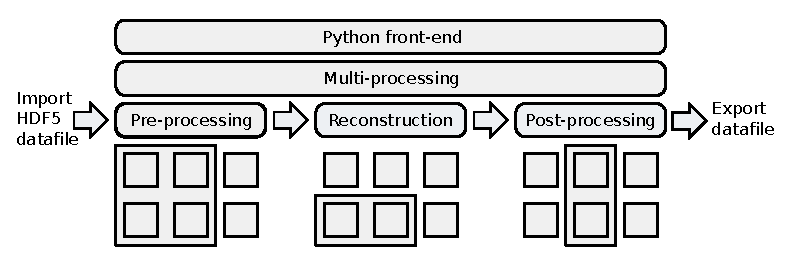
\includegraphics[width=\textwidth]{figs/framework.eps}
\caption{TomoPy framework. The analysis chain is divided into pre-processing, reconstruction and post-processing modules. Any method or a collection of methods in any language can be hooked to one of these modules without compromising the modularity. A Python front-end is used to interface these modules and interact with the user. A customizable Python based multiprocessing interface is provided for time consuming computations.}
\label{fig:Framework}
\end{figure}

\begin{figure}
\centering
\includegraphics[width=\textwidth]{figs/ring_removal.eps}
\caption{Reconstructed images before (a) and after (b) the combined wavelet-Fourier method for stripe removal is applied on normalized data.}
\label{fig:ProcessRing}
\end{figure}

\begin{figure}
\centering
\includegraphics[width=\textwidth]{figs/phase_retrieval.eps}
\caption{The phase-contrast projection data (a). Recovered phase image obtained with the single-step phase retrieval method (b). The corresponding reconstructed images with and without phase retrieval is applied (c), (d).}
\label{fig:ProcessPhase}
\end{figure}

\begin{figure}
\centering
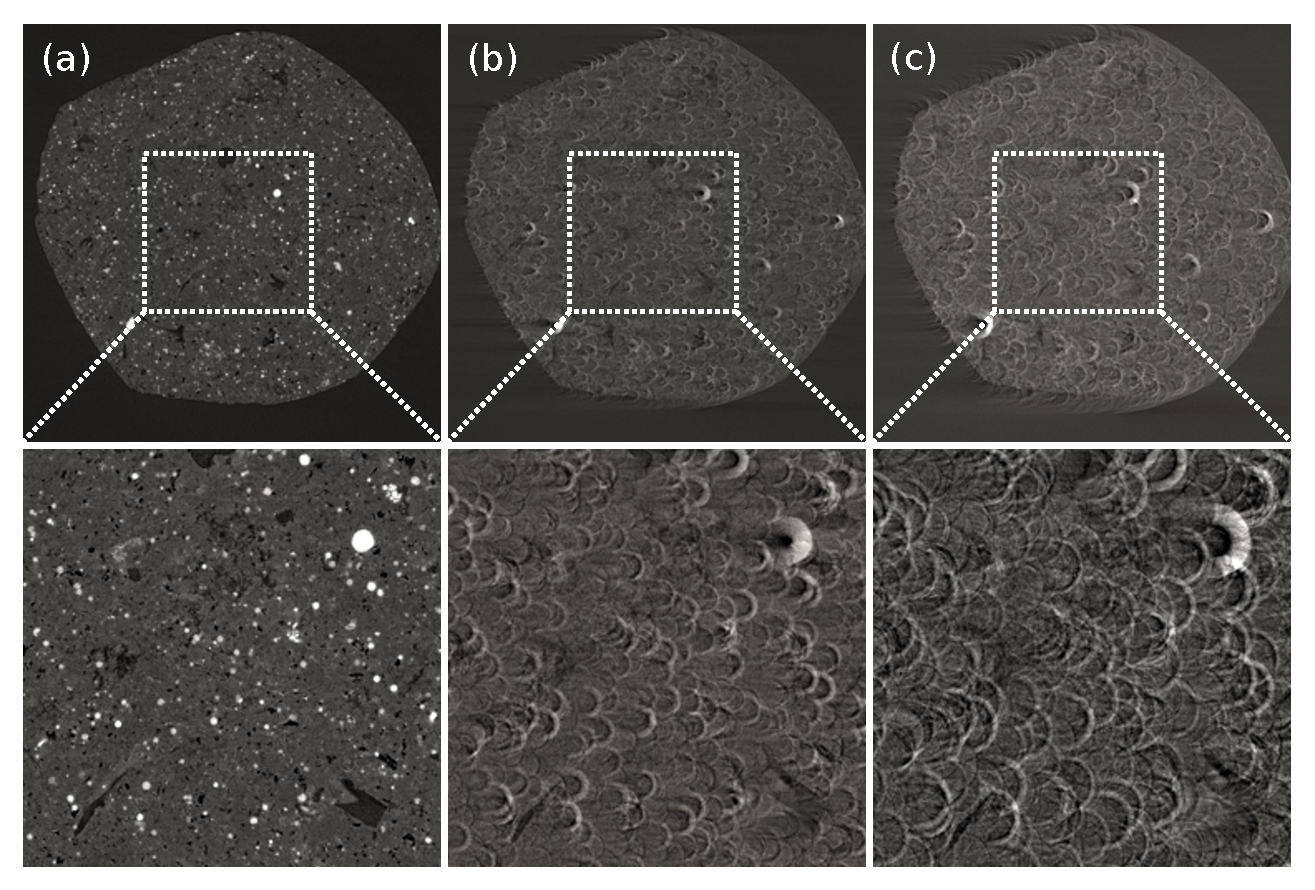
\includegraphics[width=\textwidth]{figs/center_optimize.eps}
\caption{The reconstructed images obtained with different centers of rotations: (a) Correct center, (b) 16 pixels  off-center horizontally, (c) 32 pixels off-center horizontally.}
\label{fig:OptimizeCenter1}
\end{figure}

\begin{figure}
\centering
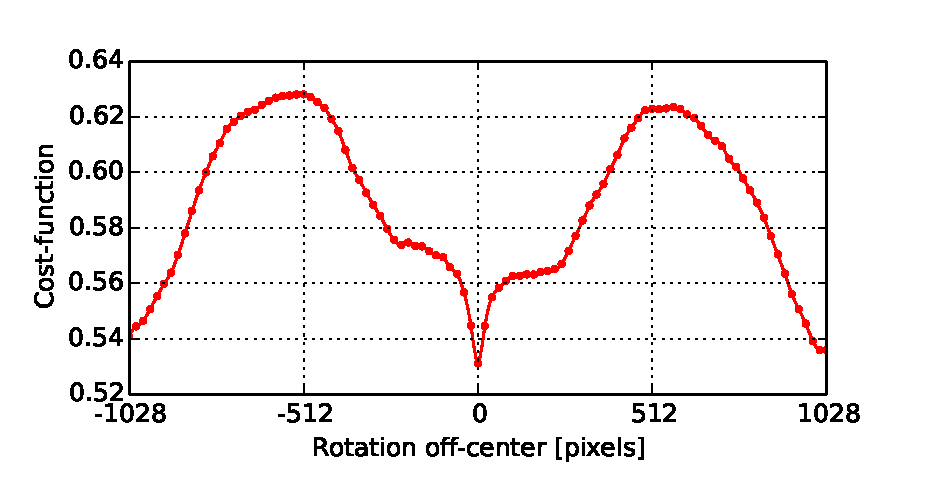
\includegraphics[width=\textwidth]{figs/center_costfunc.eps}
\caption{Plot of Shannon entropy as a function of different rotation centers. }
\label{fig:OptimizeCenter2}
\end{figure}

 

\end{document}                    % DO NOT DELETE THIS LINE
%%%%%%%%%%%%%%%%%%%%%%%%%%%%%%%%%%%%%%%%%%%%%%%%%%%%%%%%%%%%%%%%%%%%%%%%%%%%%%

